\q{13}{YouTable} \\ 

You are interested in finding out who the most popular YouTube content producers in the United States are. Your colleague used the YouTube online statistics API to find out the top 250 YouTubers in the United States as of August 2018, based on total number of video views. The first few rows of her dataset {\tt yt} are shown below. 

\begin{center}
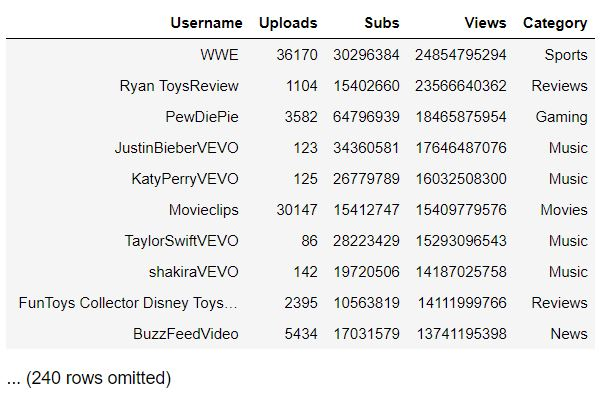
\includegraphics[scale=0.9]{yt_with_reviews.JPG}
\end{center}

In the table above, the entries in the columns \textbf{Username} and \textbf{Category} are of type {\tt string} while the entries in all other columns are of type {\tt int}. \textbf{Uploads} corresponds to number of video uploads per artist, \textbf{Subs} is number of active subscribers, and \textbf{Views} is total amount of views in all the videos a YouTube artist has released.

Fill in the blanks of the Python expressions to compute the described values. You must use only the lines provided to get full credit.The  last  line  of  each  answer  should  evaluate  to  the  value described.   Assume  that  the  statements {\tt import numpy as np} and {\tt from datascience import *} have  been executed.  You may enter anything you would like in the blanks below, but you may not add code outside of the blanks.

\begin{enumerate}

\subq{1} The total number of YouTubers in this table who have more than 1000 video uploads.\\

\lstinline{yt.________________________________________________________________________________} \\ \\
\solution{
\lstinline{yt.where('Uploads', are.above(1000)).num_rows}
}

\subq{2} You realize that the music video streaming platform VEVO contributes a lot of the top US YouTube artist accounts like "TaylorSwiftVEVO" and "shakiraVEVO". Create a table that only contains channels from VEVO, with the artists with the most subscribers at the top.\\

\lstinline{yt._________________________________________________________________________________} \\ \\
\solution{
\lstinline{yt.where('Username', are.containing('VEVO')).sort('Subs', descending=True)} \\ \\
}

\subq{3} You are interested in finding the category (ex. Sports, Music, News) with the largest average number of subscribers. Fill in the lines below so that the last line evaluates to said category.

\lstinline{only_sub_and_cat = yt.______________________________________________________________} \\ \\
\lstinline{only_sub_and_cat.___________________________________________________________________} \\ \\
\solution{
\lstinline{only_sub_and_cat = yt.select('Category', 'Subs')} \\ \\
\lstinline{only_sub_and_cat.group(0, np.mean).sort(1, descending = True).column(0).item(0)} \\ \\ 
Many people used take incorrectly. Remember take expects an array of row indicies to take from the table. 
}


\subq{3} Your friend proposes that a more effective popularity metric for YouTube content creators might be view count per video upload. Create a table with one column that contains only the usernames of the 5 top US YouTubers, sorted by highest view count per video upload.\\ \\
\lstinline{views_per_upload  = ____________________________________________________________________} \\ \\
\lstinline{yt_new_metric =  yt.with_column(________________________________________________________)} \\ \\
\lstinline{yt_new_metric.__________________________________________________________________________}\\ \\
\solution{
\lstinline{views_per_upload = yt.column('Views')/yt.column('Uploads')} \\ \\
\lstinline{yt_new_metric = yt.with_column('views_per_upload', views_per_upload)} \\ \\
\lstinline{yt_new_metric.sort('views_per_upload', descending=True).take(np.arange(5)).select('Username')}}
\\


In addition to the top 250 US YouTube accounts table from before, your friend finds a second table for the top 250 UK (United Kingdom) YouTube accounts, sorted by subscriber count. The first few rows of the {\tt yt\_uk} table are shown below. \\

\begin{center}
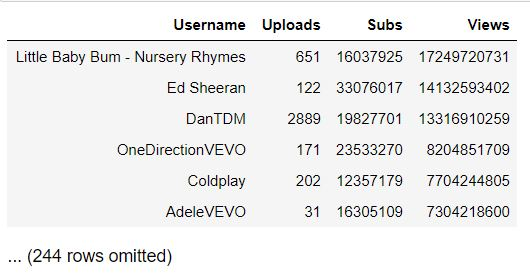
\includegraphics[scale=0.9]{youtubers_tbl_uk.JPG}
\end{center}

\subq{4} Find the number of YouTubers that are \textbf{only present in one} of the top 250 subscriber lists between the two countries. \\

\lstinline{num_youtubers_in_both =__________________________________________________________________} \\ \\
\lstinline{__________________________________________________________________________________________} \\ \\
\solution{
\lstinline{num_youtubers_in_both = yt_uk.join('Username', yt)} \\ \\
\lstinline{yt.num_rows + yt_uk.num_rows - 2*num_youtubers_in_both.num_rows} \\ \\
}
\end{enumerate}
